\documentclass[11pt]{article}

\usepackage{subfigure}
\usepackage{graphicx}
\usepackage{mathtools}
\graphicspath{{img/}{../img/}}

\usepackage{luatexja-fontspec}
\setmainjfont{SimSun}
\title{\textbf{Online Education Documentation}}
\author{Jack Wan}

\begin{document}


\maketitle
\newpage

\section{数据库设计}
\subsection{实体关系图}
整个项目的实体关系图见Figure~\ref{fig:ER-diagram}。
\subsection{表设计}
整个项目的详细数据库表设计见Figure~\ref{fig:database-tables}。

\begin{figure}[h]
  	\includegraphics[width=\linewidth]{img/ER-diagram.pdf}
  	\caption{实体关系图设计}
  	\label{fig:ER-diagram}
\end{figure}

\begin{figure}[h]
  	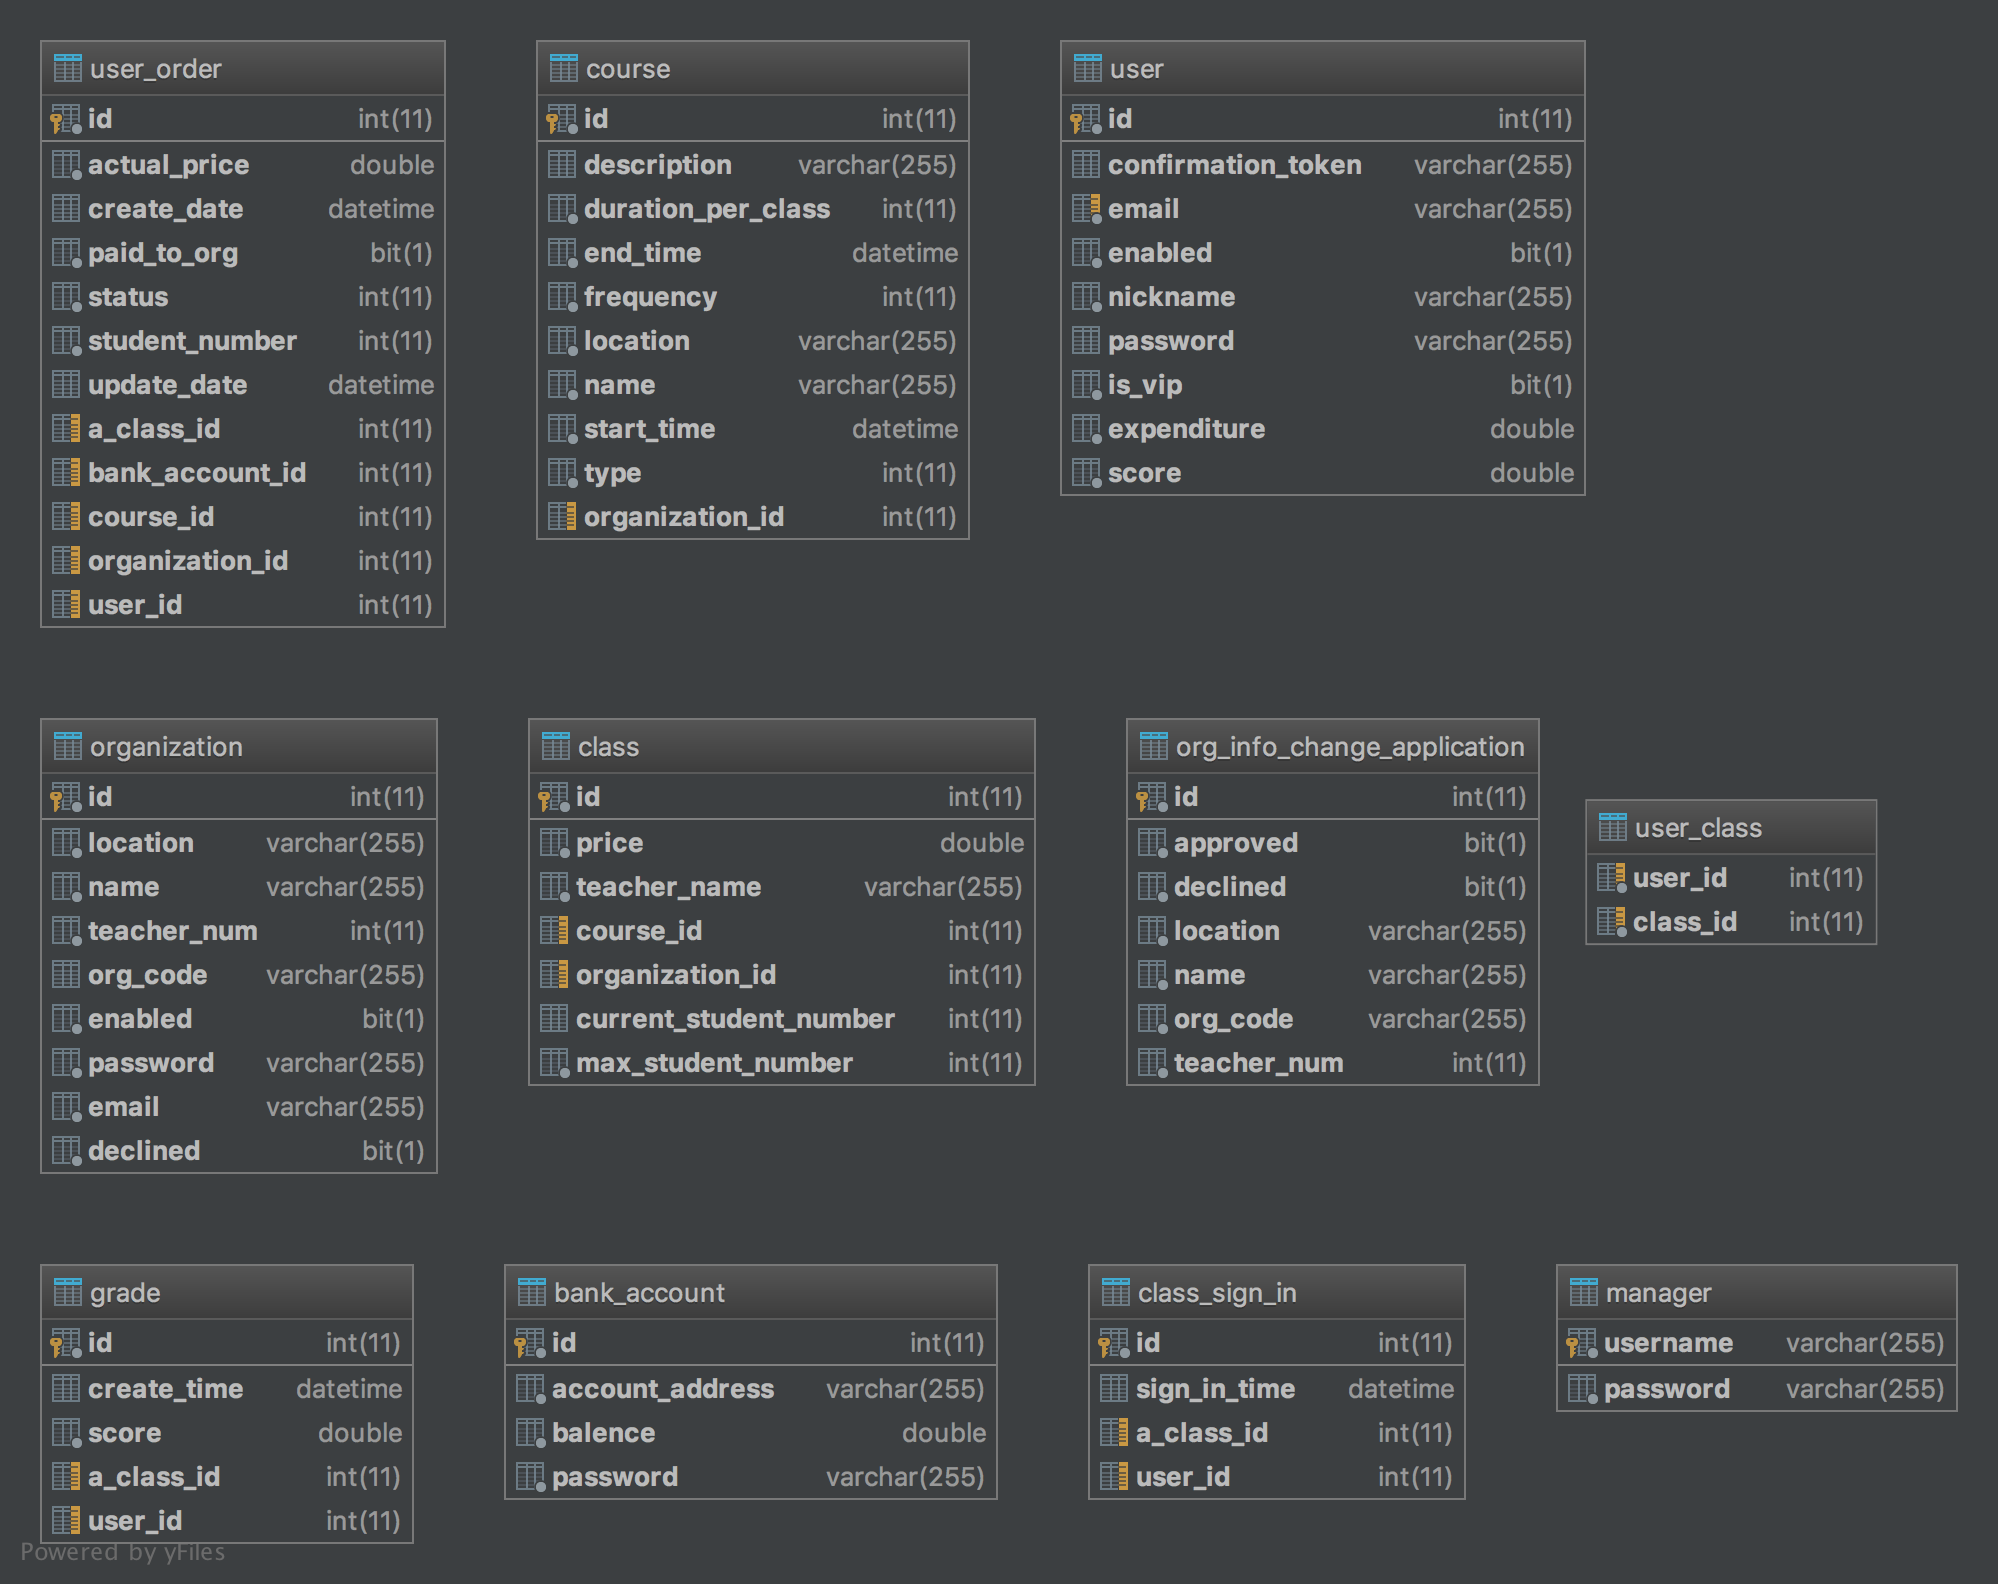
\includegraphics[width=\linewidth]{img/oleducation-tables.png}
  	\caption{数据库表设计}
  	\label{fig:database-tables}
\end{figure}


\section{架构设计}
\subsection{工程的项目结构截图}
前后端的文件结构如Figure~\ref{fig:structure}所示。

\begin{figure}[h]
    \centering 
    \subfigure[后端结构]{
        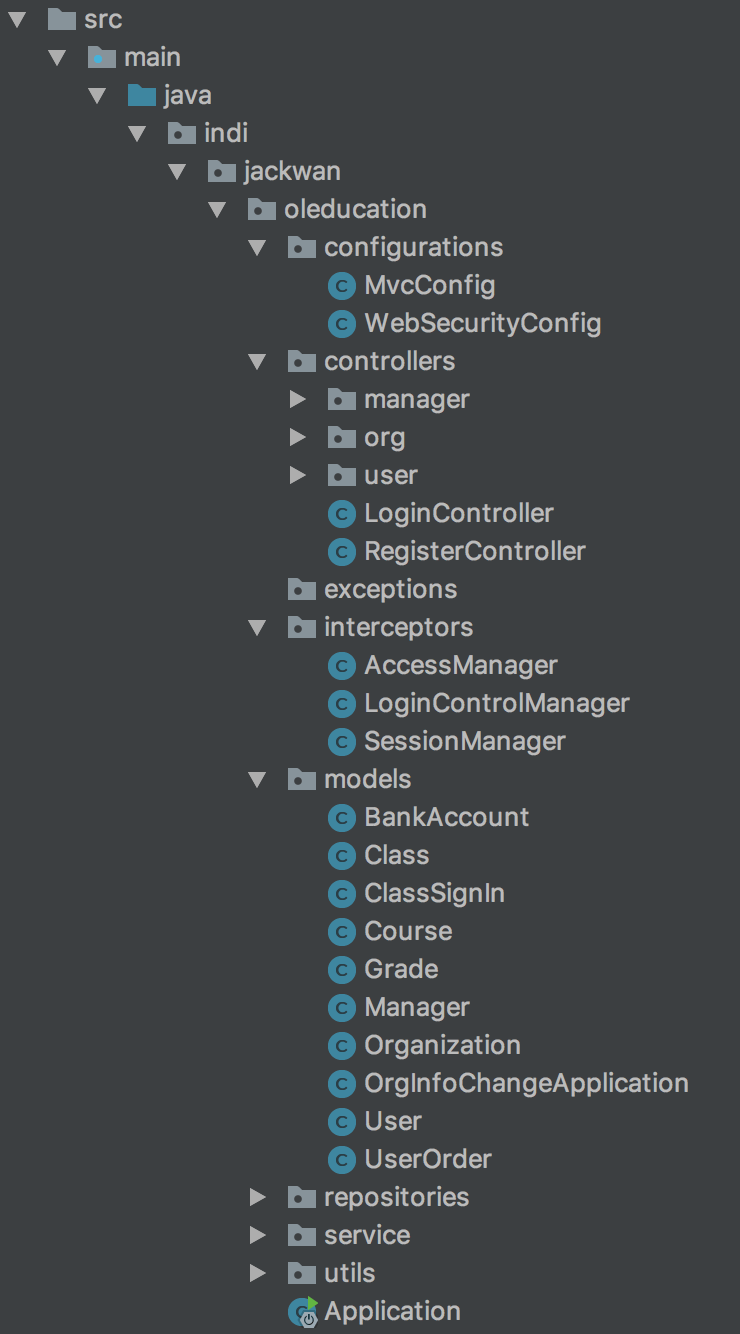
\includegraphics[width=0.48\columnwidth]{img/Backend-Structure.png} 
    } 
    \subfigure[前端结构] {
        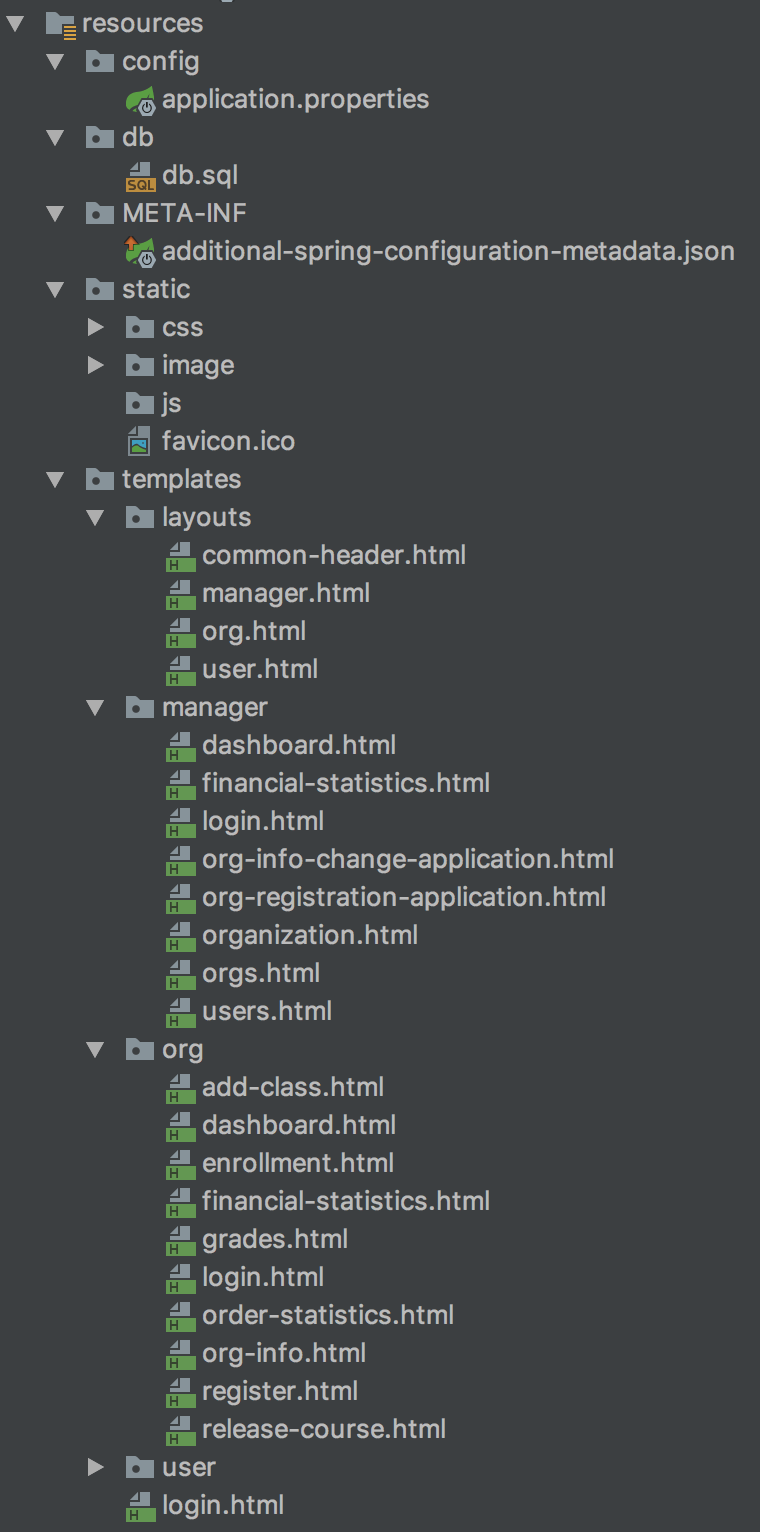
\includegraphics[width=0.43\columnwidth]{img/Frontend-Structure} 
    }
    \caption{项目结构} 
    \label{fig:structure}
\end{figure}

\subsection{后端框架}
此次项目的后端采用了Spring Boot + Spring MVC + Spring Data + Gradle的框架,实现了零XML配置,以及非常便捷的部署流程。

\subsection{前端框架}
此次项目的前端主要采用了Thymeleaf + Bootstrap + JQuery的传统框架,其中Thymeleaf是一种可直接在浏览器渲染的模版引擎。详细的依赖图见Figure~\ref{fig:frontend-dependency}。

\begin{figure}[h]
  	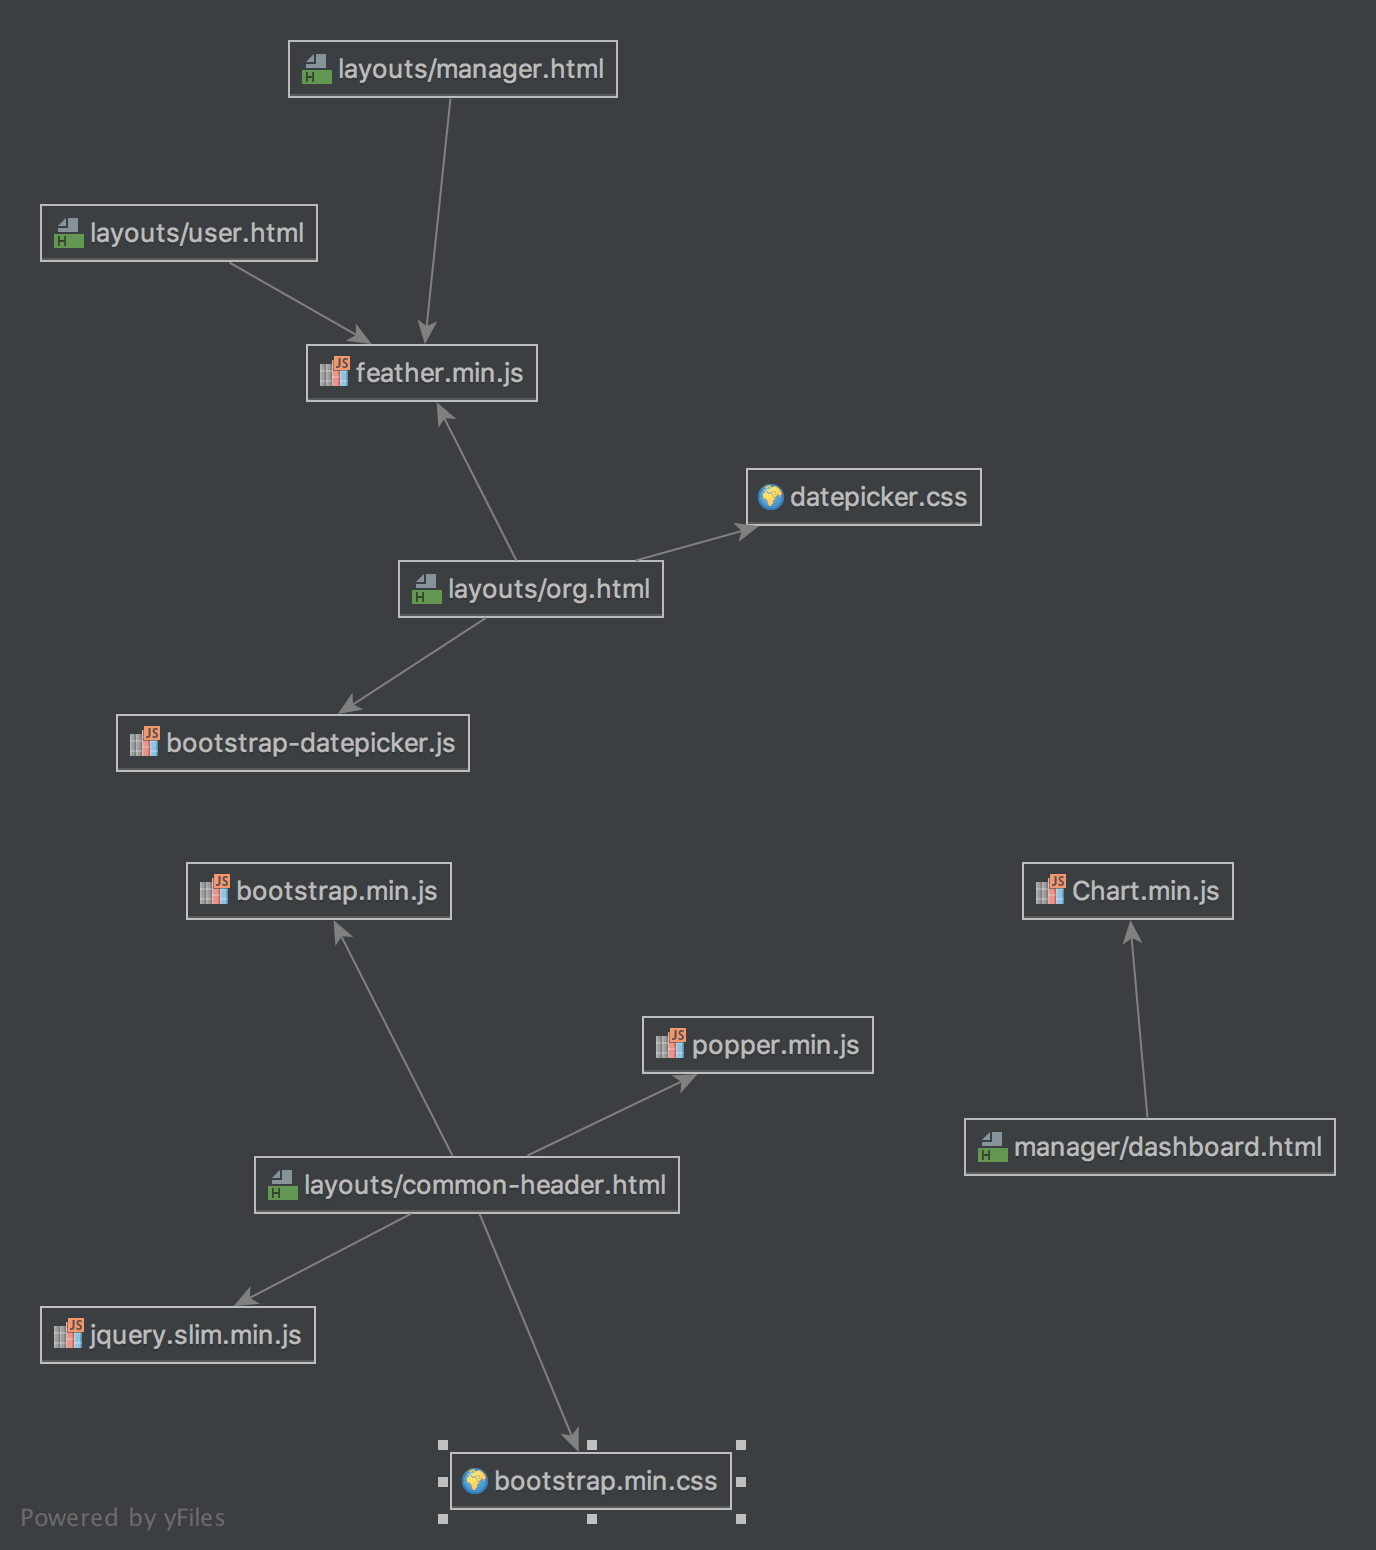
\includegraphics[width=\linewidth]{img/Front-End-Framework.png}
  	\caption{前端框架}
  	\label{fig:frontend-dependency}
\end{figure}

\section{类设计}
\subsection{各包的类设计}
\begin{enumerate}
    \item \textbf{configurations} 包含两个类,分别是\texttt{MvcConfig}和\texttt{WebSecurityConfig},主要的指责是配置Spring的环境,包括权限管理、以及路由管理等。
    \item \textbf{controllers} 包含了Spring MVC框架中所有的控制器类。
    \begin{enumerate}
      \item \textbf{manager} 包含了所有对用以\texttt{/manager}为首请求的控制器类。其下一共有4个类,分别是\texttt{ManagerController},\texttt{ManagerOrganizationController},\texttt{ManagerOrgInfoController},\texttt{ManagerUserController}。类的名字已经显示了此类的作用,比如,\texttt{ManagerUserController}就负责Manager对User的相关请求的处理。
      \item \textbf{org} 包含了所有对用以\texttt{/org}为首请求的控制器类。其下一共有7个类,分别是\texttt{OrgClassController},\texttt{OrgController},\texttt{OrgCourseController},\texttt{OrgEnrollmentController},\texttt{OrgGradesController},\texttt{OrgInfoController}和\texttt{OrgStatisticsController}。同样,类的名字暗示了类的职责。
      \item \textbf{user} 包含了所有对用以\texttt{/user}为首请求的控制器类。
      \item \textbf{LoginController} 对所有用户的登录做处理。其下一共有8个类,分别是\texttt{UserClassController},\texttt{UserController},\texttt{UserCourseController},\texttt{UserInfoController},\texttt{UserMembershipController},\texttt{UserOrderController},\texttt{UserPrivilegeController}和\texttt{UserScoreController}。再一次,类的名字暗示了类的职责。比如,\texttt{UserCourseController}负责对User请求查看Courses的处理,\texttt{UserMembershipController}负责对User取消,查看自己当前的VIP状态的处理。
      \item \textbf{RegisterController} 对普通学员和组织的注册申请做处理。
    \end{enumerate}
    \item \textbf{interceptors} 是对J2EE中\texttt{Filter}的替代,此包中定义了3个Interceptor,分别是\texttt{AccessManager},负责对三种不同的网站用户类型做权限管理,\texttt{LoginController},负责控制对未登录用户的权限管理,\texttt{SessionManager},负责对Session生命周期的管理。
    \item \textbf{models} 定义了所有的实体类,包括\texttt{BankAccount},\texttt{Class},\texttt{ClassSignIn},\texttt{Course},\texttt{Grade},\texttt{Manager},\texttt{Organization},\texttt{OrgInfoChangeApplication},\texttt{User},\texttt{UserOrder}。
    \item \textbf{repositories} 定义了所有基于Spring Data的Repository类,是对底层SQL查询的一层封装。
    \item \textbf{service} 定义了所有核心业务逻辑,其中一共有11个类,分别是\texttt{ClassService},\texttt{CourseService},\texttt{EmailService},\texttt{ManagerService},\texttt{OrderService},\texttt{OrgCourseService},\texttt{OrgInfoChangeApplicationService},\texttt{OrgService},\texttt{PaymentService},\texttt{UserService}和\texttt{VipService}。每个Service可能持有一个或多个Repository的引用,用来进行对数据库的调用。
    \item \textbf{utils} 其他的工具类,比如生成7位机构码以及其他各种\texttt{Enum}类型。
    \item \textbf{Application} 是整个Web应用的入口。
\end{enumerate}

\subsection{前端页面设计}
\begin{enumerate}
  \item \textbf{\texttt{/login}} 三种用户皆通过此页面导航至对应的页面。
  \item \textbf{\texttt{/user}}
    \begin{enumerate}
      \item \texttt{/} 用户的主页面,对应了Dashboard,显示了该用户当前所在的课程信息。
      \item \texttt{/login} 用户的登录入口。
      \item \texttt{/logout} 所有类型用户的登出入口。
      \item \texttt{/orders} 显示了该用户当前的订单信息,包括订单号,金额,课程号,时间,订单状态等信息。
      \item \texttt{/courses} 显示了当前此平台所有的课程信息,包括开课日期,现有人数,最大容量等。
      \item \texttt{/info} 显示了当前用户的具体信息,以及修改对应信息的入口。 
      \item \texttt{/privilege} 显示了当前该用户的会员等级,以及对应的特权(如果该用户不是VIP则不显示)。 
      \item \texttt{/score} 显示了积分系统的运行规则以及该用户当前的可用积分。 
      \item \texttt{/membership} 提供了取消VIP资格的入口。
    \end{enumerate}
  \item \textbf{\texttt{/org}}
    \begin{enumerate}
      \item \texttt{/} 机构的Dashboard,显示了该机构现有的所有课程。
      \item \texttt{/login} 机构的登录入口。
      \item \texttt{/info} 显示机构信息,提交修改机构信息申请的入口。
      \item \texttt{/course} 发布课程的入口。
      \item \texttt{/enrollment} 线下报名的入口。
      \item \texttt{/grades} 登记成绩和签到的入口。
      \item \texttt{/order-statistics} 查看该机构所有的订单,并提供相关的统计信息。
      \item \texttt{/financial-statistics} 查看该机构的财务统计信息。
    \end{enumerate}
  \item \textbf{\texttt{/manager}}
    \begin{enumerate}
      \item \texttt{/} 管理人员的Dashboard,提供了整个平台的财务统计信息,如营业额,盈利额,可流通资金等。
      \item \texttt{/login} 管理人员的登录入口。
      \item \texttt{/org-registration-application} 管理员审核机构注册申请的页面,提供了机构注册申请的详细信息。
      \item \texttt{/org-info-change-application} 管理员审核机构修改信息申请的页面,提供了信息申请的详细信息。
      \item \texttt{/organizations} 管理员可通过此入口查看所有的机构信息以及对应的统计信息。
      \item \texttt{/users} 管理员可通过此入口查看所有的用户信息以及对应的统计信息。
    \end{enumerate}
\end{enumerate}

\section{其他}


\subsection{开发环境}
\begin{enumerate}
  \item \textbf{服务器} 由于此项目采用的是\textbf{Spring Boot 2.0},所以对应的服务器是内置的\textbf{Tomcat}服务器
  \item \textbf{数据库} \textbf{MySQL Ver 14.14 Distrib 5.7.16}
  \item \textbf{IDE} \textbf{IntelliJ IDEA}
\end{enumerate}


\subsection{心得体会}
\begin{enumerate}
  \item 前端组件还可以更加美观,用户体验可以更加自然。
  \item 后端数据库的查询还可以做更好的优化。
  \item 项目里程碑的设立非常重要,有一个好的个人软件习惯往往能决定整个工程的质量。
  \item 框架的使用会在很大程度上简化开发过程,但是学习成本也不可忽视,在同样的时间内,延用旧技术的人可能已经完成了四分之一,但是学习使用新技术的人可能才刚刚写出Hello World。我属于后者,这个项目尽全力向产业界前沿靠拢,采用了Spring Boot + Gradle + Spring MVC的架构,使得整个项目的配置没有用到任何XML。个人认为,XML配置文件繁琐的语法决定了其必将会被更高层次的封装所替代的命运。尽管如此,这个项目还有很多可以提高的地方,关于框架这一点上,Spring Security会是另一个很好的选择。
  \item 前端仍有很多重复代码,比如各种表格的重复出现,后期可以通过将其组件化来进行完善。采用最新的前端框架也是另外一个选项,但就像刚才所说的,昂贵的学习成本以及集成难度是这个过程最大的阻力。
  \item 测试不完善,敏捷开发及TDD并没有得到落实,测试用例的缺少也使得持续集成成为泡影,整个工程的质量可以说是没有任何硬性保障。作为一个学期大作业,我认为这是可以理解的,但如果我们用工业界的标准来要求自己,就会连将其开源的勇气都没有。但是我想说的是,这样的意识是宝贵的,在以后的代码过程中,也要时刻有这样的意识。
\end{enumerate}

\end{document}